% Single manuscript. All sections, tables and the method schematic live here.
% Data provenance and remaining experiments are in author_notes/, not this paper.
\documentclass{article}
\usepackage{iclr2027_conference,times}
\usepackage[T1]{fontenc}
\usepackage{amsmath,amssymb,amsthm,booktabs,tabularx,array,multirow}
\usepackage{graphicx,microtype,url,hyperref}
\usepackage{tikz}
\usetikzlibrary{arrows.meta,positioning,fit,calc}
\newcommand{\method}{\textsc{Visual Lens}}
\newcommand{\R}{\mathbb{R}}
\newcommand{\Sset}{\mathcal{S}}
\newcommand{\Qset}{\mathcal{Q}}
\newcommand{\Lset}{\mathcal{J}}
\newcommand{\tr}{\operatorname{tr}}
\newcommand{\diag}{\operatorname{diag}}
\newcommand{\sm}{\operatorname{softmax}}
\newcommand{\TopEig}{\operatorname{TopEig}}
\newtheorem{proposition}{Proposition}
\title{A Learned Visual Lens: Low-Rank State\\ Adaptation for Vision--Language Models}
\author{Anonymous authors}
% \iclrfinalcopy  % Leave commented for double-blind review.
\begin{document}
\maketitle

\begin{abstract}
A frozen vision--language model can adapt to a new visual domain without learning a weight update. In a four-event disaster-assessment comparison, a controller with 1,024 learned coefficients attains 32.08\% mean macro-F1, compared with 29.86\% for a 10.1-million-parameter LoRA adapter using the same labeled support. This contrast motivates a learned visual lens: a small transformation of the internal states through which the model processes image evidence. We estimate a linear subspace from the second moment of correct-answer gradients, then fit an identity-initialized, norm-bounded residual on selected visual key/value states. The backbone and subspace remain fixed during fitting, and one controller serves all subsequent queries from the target domain. Experiments span disaster assessment, histopathology, execution verification, and manipulation question answering. Rank-matched random and centered-gradient controls establish the value of correctness-sensitive directions on the disaster task, while medical and robotic results reveal substantial variation in the advantage over weight adaptation. Mechanism probes further separate gradient-energy coverage, signed directional agreement, and intervention location: shared gradient energy alone does not determine the utility of an internal correction. A learned visual lens thus offers a compact form of few-shot adaptation and exposes which parts of the adaptation problem remain outside the tested visual-state restriction.
\end{abstract}



\section{Introduction}
\label{sec:intro}
\textbf{More adaptable parameters need not yield a better few-shot adaptation.} On four BRIGHT disaster events, we compare two ways to specialize the same vision--language model (VLM) using 24 labeled buildings per event. A rank-16 LoRA adapter learns 10,092,544 parameters and obtains 29.86\% mean macro-F1. A residual controller restricted to visual attention states learns only 1,024 coefficients and obtains 32.08\% (Figure~\ref{fig:observation}). The small controller improves on the frozen model in all four events, although LoRA remains stronger in two. The result challenges a capacity-first approach to this deployment setting: the location and structure of an update matter alongside its size.

\begin{figure}[!ht]
\centering
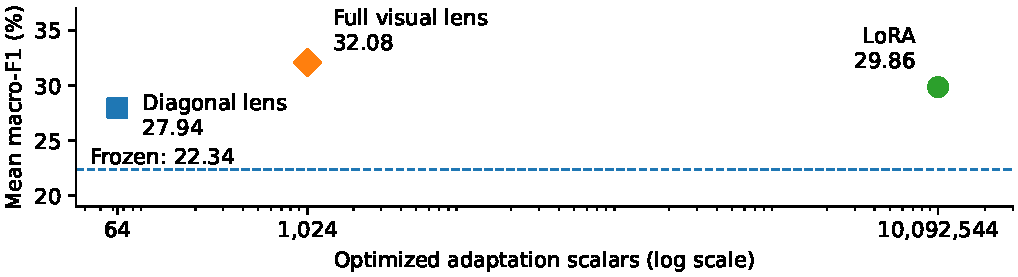
\includegraphics[width=\linewidth]{figures/fig1_observation.pdf}
\caption{\textbf{A small internal correction competes with a much larger weight update.} Qwen2.5-VL-7B, four BRIGHT events, support24/query300, one support set per event. The horizontal axis counts optimized variables; the dashed line is frozen inference. Full-lens macro-F1 exceeds LoRA with 9,856 times fewer learned scalars. Basis storage and compute are accounted for separately.}
\label{fig:observation}
\end{figure}



The practical question is therefore \emph{what should a few labeled examples be allowed to change?} Disaster assessment makes this pressure concrete: a handful of labeled buildings must support decisions across a new event, with paired optical and post-event observations \citep{chen2025bright}. A weight adapter offers broad flexibility. We instead learn a small correction at the internal states carrying the visual input.

We call this correction a \emph{learned visual lens}. It leaves the images and backbone weights unchanged and transforms selected visual states inside the language decoder. The design preserves the base computation, identifies task-sensitive directions, and fits a bounded correction within those directions.

We instantiate this design in two stages. First, gradients of the correct support answers identify a low-dimensional subspace of visual key/value states. We use their uncentered second moment, retaining variation that a single mean direction discards. Second, a small matrix learns a residual transformation inside that fixed subspace. On paired disaster images, the direct intervention is restricted to post-event visual tokens. On single-image tasks, it covers the image-token group. The resulting controller is fitted once per domain and reused across its query examples.

The distinctive choice is \emph{support-conditioned visual-state restriction}. Whereas LoRA learns weight deltas and representation finetuning learns internal interventions \citep{hu2022lora,wu2024reft}, we use answer sensitivity to determine the permitted visual directions. Correctness-derived KV subspaces also appear in self-policy distillation \citep{hao2026spd}; here they support a reusable deployment-time residual instead of a synthetic-data generation process.

The full lens improves primary BRIGHT macro-F1 by 9.74 points over frozen inference with 9,856 times fewer optimized variables than LoRA. Additional backbones and tasks test the same restriction. These experiments reveal a second observation: shared support/query gradient energy does not reliably track a correction's usefulness. Signed gradient statistics and projection-site interventions help explain the difference.

Our contributions are threefold. (1) We introduce a correctness-guided visual lens that learns a bounded low-rank state correction from labeled target support while keeping the backbone fixed. (2) We establish its accuracy--adaptation-size trade-off on BRIGHT and evaluate the same restriction across six VLM backbones and three application families. (3) We use basis, optimization, and projection-site controls to distinguish shared gradient directions from corrections realizable by the tested controller.

\section{A learned visual lens}
\label{sec:method}
\subsection{Support-conditioned adaptation}
A target domain $e$ provides labeled support $\Sset_e=\{(x_i,y_i)\}_{i=1}^{N}$ and disjoint queries $\Qset_e$. The input $x_i$ contains an image or image pair and a question; $y_i$ is a candidate answer string. We start from a pretrained VLM $f_\theta$. All competing methods within an experiment share that checkpoint and the same support/query identifiers. Our setting is supervised few-shot adaptation at deployment: support labels train the lens, which is fixed before query prediction.

For a selected decoder projection $j=(\ell,t)$, $t\in\{K,V\}$, let $Z_{i,j}\in\R^{T_i\times d_j}$ be the projection output before head reshaping and any subsequent positional transformation. A binary row mask $M_i$ selects the relevant visual tokens. We intervene on these projection outputs, not on an external feature--label memory. The ordinary attention computation still uses queries, keys, and values; modifying visual K/V changes the information available to later tokens through that computation.

\begin{figure}[t]
\centering
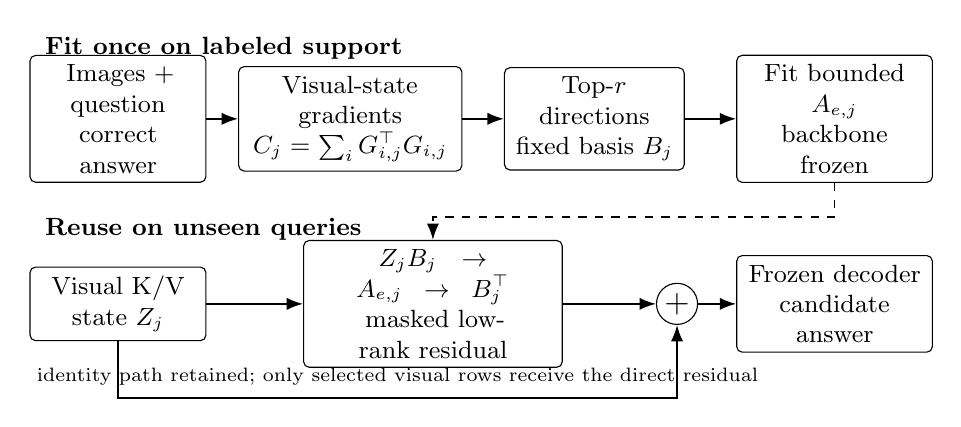
\begin{tikzpicture}[x=1cm,y=1cm,>=Latex,
 box/.style={draw,rounded corners=2pt,align=center,font=\small,minimum height=.85cm},
 lab/.style={font=\small,align=center},arr/.style={->,line width=.65pt}]
\node[lab,anchor=west] at (0,3.25) {\textbf{Fit once on labeled support}};
\node[box,text width=2.0cm] (sup) at (1.05,2.35) {Images + question\\correct answer};
\node[box,text width=2.6cm] (grad) at (4.0,2.35) {Visual-state gradients\\$C_j=\sum_i G_{i,j}^{\top}G_{i,j}$};
\node[box,text width=2.05cm] (basis) at (7.1,2.35) {Top-$r$ directions\\fixed basis $B_j$};
\node[box,text width=2.25cm] (fit) at (10.15,2.35) {Fit bounded $A_{e,j}$\\backbone frozen};
\draw[arr] (sup)--(grad);\draw[arr] (grad)--(basis);\draw[arr] (basis)--(fit);
\node[lab,anchor=west] at (0,.95) {\textbf{Reuse on unseen queries}};
\node[box,text width=2.0cm] (z) at (1.05,0) {Visual K/V\\state $Z_j$};
\node[box,text width=3.05cm] (res) at (5.05,0) {$Z_jB_j\ \to\ A_{e,j}\ \to\ B_j^{\top}$\\masked low-rank residual};
\node[draw,circle,font=\large,inner sep=1pt] (sum) at (8.15,0) {$+$};
\node[box,text width=2.25cm] (out) at (10.15,0) {Frozen decoder\\candidate answer};
\draw[arr] (z)--(res);\draw[arr] (res)--(sum);\draw[arr] (sum)--(out);
\draw[arr] (z.south)--++(0,-.72)-|(sum.south);
\draw[arr,dashed] (fit.south)--(10.15,1.1)--(5.05,1.1)--(res.north);
\node[lab,font=\scriptsize] at (4.6,-.93) {identity path retained; only selected visual rows receive the direct residual};
\end{tikzpicture}
\caption{\textbf{A lens is an operator, not a replacement model.} Correct-answer gradients select a linear visual-state subspace. A bounded matrix is then fitted inside that subspace and reused across query images. The dashed arrow transfers the fitted state; solid arrows denote computation. The original path remains present. Each query creates its own activations, transformed by the same domain-specific lens.}
\label{fig:method}
\end{figure}

\subsection{Select directions using correct-answer sensitivity}
\label{sec:basis}
We restrict the autoregressive training loss to the correct answer span $\mathcal T_i$:
\begin{equation}
 \mathcal L_i=-\frac{1}{|\mathcal T_i|}\sum_{u\in\mathcal T_i}
 \log p_\theta(y_{i,u}\mid x_i,y_{i,<u}),\qquad
 G_{i,j}=\left[\frac{\partial\mathcal L_i}{\partial Z_{i,j}}\right]_{M_i}.
 \label{eq:grad}
\end{equation}
Here $G_{i,j}$ contains only selected visual rows. We construct a separate second moment for each projection:
\begin{equation}
 C_j=\frac1N\sum_{i=1}^{N}G_{i,j}^{\top}G_{i,j},\qquad
 B_j=\TopEig_r(C_j),\qquad B_j^{\top}B_j=I_r.
 \label{eq:basis}
\end{equation}
The columns of $B_j$ are linear sensitivity directions. Opposing gradients can occupy the same direction: squaring before aggregation retains its energy even when the average cancels. Coefficient fitting determines how to combine these directions.

\begin{proposition}[Support-gradient energy retention]
For $C\succeq0$ and $B\in\R^{d\times r}$ with $B^\top B=I_r$,
\begin{equation}
 \max_{B^\top B=I_r}\tr(B^\top CB)=\sum_{k=1}^{r}\lambda_k(C).
 \label{eq:energy}
\end{equation}
The leading eigenvectors attain the maximum. For Equation~\ref{eq:basis}, the objective equals $N^{-1}\sum_i\|G_iB\|_F^2$.
\end{proposition}
This classical characterization selects the subspace retaining the most observed support-gradient energy; Appendix~\ref{app:proof} gives the proof. Query transfer and downstream utility remain empirical questions.

\subsection{Fit a bounded residual inside the selected subspace}
The full lens applies
\begin{equation}
 \widetilde Z_{i,j}=Z_{i,j}+M_i\odot\left[(Z_{i,j}B_j)A_{e,j}B_j^\top\right],
 \qquad A_{e,j}=\frac{\alpha R_{e,j}}{1+\|R_{e,j}\|_F}.
 \label{eq:lens}
\end{equation}
Only $R_{e,j}\in\R^{r\times r}$ is trainable; the mask broadcasts over channels. The diagonal variant uses $A_{e,j}=\diag(\alpha\tanh a_{e,j})$ instead of full mixing. Both start at zero, recovering the unmodified model.

The residual preserves the base activation and its orthogonal component. For any selected row $z$, $(\widetilde z-z)(I-B_jB_j^\top)=0$, and
\begin{equation}
 \|A_{e,j}\|_2<\alpha,\qquad
 \|\widetilde Z_{i,j}-Z_{i,j}\|_F
 \leq\alpha\|M_i\odot(Z_{i,j}B_j)\|_F.
 \label{eq:bound}
\end{equation}
The bound controls the local residual. Text rows receive no direct write; attention to the edited visual states changes their downstream representations and the answer.

\paragraph{Fitting and reuse.}
Let $\phi_e$ collect the raw matrices $R_{e,j}$. We optimize
\begin{equation}
 \min_{\phi_e}\ \sum_{i=1}^{N}w_i\mathcal L_i(f_{\theta,B,\phi_e})
 +\lambda\sum_{j\in\Lset}\|R_{e,j}\|_F^2,
 \label{eq:fit}
\end{equation}
with Adam and gradient clipping. The executed scaling is $w_i=1/N$ on BRIGHT and $w_i=1$ on single-image tasks. Each update accumulates all support examples. Queries then reuse $B_j,A_{e,j}$ without further fitting or support context. Two-layer K/V full and diagonal lenses learn $4r^2$ and $4r$ scalars: 1,024 and 64 for $r=16$. Storage also includes the fixed bases.

\paragraph{Computation.}
Extraction uses one backward pass per support example and an eigendecomposition per module. Query inference adds $O(Tdr+Tr^2)$ work per full-lens module, or $O(Tdr)$ for a diagonal lens, without extra tokens or retrieval.



\section{Experimental design}
\label{sec:setup}
We test the adaptation-size trade-off, the value of correctness-derived directions, and variation across tasks. The primary estimator is BRIGHT mean event macro-F1; medical and robotic tasks test transfer of the same operator.

\paragraph{Data and supervision.}
BRIGHT \citep{chen2025bright} supplies building-level pre/post observations. The four-event subset comprises Hawaii wildfire, Libya flood, Noto earthquake, and Turkey earthquake. Each event has 24 labeled support buildings, eight per damage class, and 300 balanced query buildings. Support and query tiles are disjoint. The input is a $448\times448$ building crop from each observation; only the second image's visual states are modified. The evaluated derivative is a building-classification subset of the multimodal dataset.

Camelyon17-WILDS \citep{koh2021wilds} supplies normal/tumor patches from hospital 2, with support16 and query300. The robot execution-verification data associated with Guardian/FailCoT \citep{pacaud2026guardian} comprise UR5-Fail, RoboFail, and the RoboVQA execution subset. Each uses eight support examples per class and the remaining 124, 137, or 341 examples as query. A before/after pair is vertically stitched into one image; UR5 uses its front camera. ManipBench Q1 \citep{zhao2025manipbench} uses 32 support questions and 400 queries in each of Bridge pick-and-place, DROID articulated manipulation, and DROID pick-and-place. Its four answer letters index the options of each question. These robotic evaluations measure offline visual decisions rather than closed-loop control.

\paragraph{Backbones and baselines.}
Qwen2.5-VL-7B \citep{bai2025qwen25vl} is the primary backbone. Qwen3-VL-8B and InternVL3-8B \citep{bai2025qwen3vl,zhu2025internvl3} supply additional BRIGHT and single-image task comparisons. Phi, Gemma 3 4B, and a Llama-backed LLaVA supply additional BRIGHT controls. All methods start independently from the corresponding pretrained checkpoint. Frozen inference is the unadapted reference. LoRA uses rank 16, scaling 32, dropout 0.05, and Q/K/V/O targets. Random-KV replaces the gradient basis with an orthonormal random basis while preserving the lens and fitting budget.

\paragraph{Budgets and scoring.}
The standard full lens uses $r=16$, $\alpha=3$, layers 14 and 27, four updates, learning rate 0.05, $\lambda=10^{-3}$, and clipping at 1. Guardian additionally has a fixed eight-update, learning-rate-0.01 follow-up. Primary BRIGHT LoRA uses eight optimizer updates at $10^{-4}$ with accumulation over three examples; cross-backbone BRIGHT uses $2\times10^{-4}$. Task LoRA uses four support passes at $2\times10^{-4}$, with one update per example. These share labels and examples but differ in optimizer updates and compute. Appendix~\ref{app:protocol} gives the implementation contract.

Every method scores candidates with summed answer-token log-likelihood and normalizes those scores across candidates. InternVL task examples use the explicit \texttt{Answer: <label>} span. Its single-image path uses 224 pixels and 64 visual tokens; its BRIGHT path uses 448 pixels. Inputs and scoring are identical within each method comparison. We report macro-F1, balanced accuracy (BA), and negative log-likelihood (NLL), preserving differences between hard-label and probabilistic outcomes.

\paragraph{Replication.}
The primary BRIGHT and cross-backbone comparisons use one locked support set per event. A separate compact rank-5 BRIGHT experiment repeats the lens over three support seeds against frozen inference. Camelyon, Guardian, and ManipBench compare methods over three matched support seeds, reporting sample standard deviations. Guardian queries change with the held-out support selection. Mechanism probes using query labels are separated from deployment estimates. Parameter sweeps characterize sensitivity on the evaluated sets; the primary table reports one shared configuration across events.

\section{Adaptation across visual domains}
\label{sec:results}
\subsection{A compact lens improves the primary disaster comparison}
Table~\ref{tab:main} gives the complete primary comparison. The full lens raises mean macro-F1 from 0.2234 to 0.3208 and exceeds the fixed-duration LoRA reference by 0.0222. The benefit appears on every event relative to frozen inference, but is concentrated on Libya and Turkey relative to LoRA. A diagonal lens retains most of the gain over frozen inference with only 64 coefficients, while full mixing adds 0.0414 mean F1.

\begin{table}[t]
\caption{\textbf{Primary BRIGHT results.} Qwen2.5-VL-7B; identical support24 and balanced query300 per event. BA and NLL are four-event means. The optimized-scalar count excludes fixed bases. Best values are bold; lower NLL is better.}
\label{tab:main}
\centering\small
\begin{tabular}{@{}lrrrrrrr@{}}
\toprule
Method & Hawaii & Libya & Noto & Turkey & Mean F1 & BA & NLL\\
\midrule
Frozen & .1992 & .2585 & .2087 & .2273 & .2234 & .3450 & 1.3233\\
LoRA & \textbf{.3526} & .2776 & \textbf{.3495} & .2147 & .2986 & \textbf{.3567} & \textbf{1.1276}\\
Diagonal lens & .2918 & .2560 & .2820 & .2879 & .2794 & .3442 & 1.1715\\
Full lens & .2957 & \textbf{.3739} & .3112 & \textbf{.3025} & \textbf{.3208} & .3450 & 1.1367\\
\bottomrule
\end{tabular}
\end{table}

The full lens improves macro-F1 while mean BA stays at 0.3450, close to the three-class chance rate. LoRA has slightly better mean BA and NLL. The demonstrated advantage is therefore macro-F1 per optimized adaptation variable. The complete metric profile distinguishes this gain from an improvement in every aspect of class discrimination.

\subsection{The operator transfers, but the advantage is backbone-dependent}
Table~\ref{tab:backbones} retains all additional BRIGHT backbones. The full lens leads on Qwen3-VL, InternVL3, and Gemma 3; LoRA leads on Phi, and frozen inference on LLaVA. The substantial gaps to random bases on Qwen3 and InternVL show that useful task-conditioned directions extend beyond one checkpoint.

\begin{table}[t]
\caption{\textbf{Additional BRIGHT backbones.} Four-event mean macro-F1 under support24/query300. Each row compares the same checkpoint, preprocessing, support, and query. The common generic runner uses eight LoRA updates at $2\times10^{-4}$.}
\label{tab:backbones}
\centering\small
\begin{tabular}{@{}lrrrr@{}}
\toprule
Backbone & Frozen & LoRA & Random-KV & Full lens\\
\midrule
Qwen3-VL-8B & .1667 & .2034 & .1687 & \textbf{.3492}\\
InternVL3-8B & .1848 & .1667 & .2214 & \textbf{.2860}\\
Phi & .1665 & \textbf{.2364} & .1665 & .2075\\
Gemma 3 4B & .1737 & .1970 & .1820 & \textbf{.2607}\\
Llama-backed LLaVA & \textbf{.2134} & .1667 & .1872 & .2034\\
\bottomrule
\end{tabular}
\end{table}

\subsection{Medical and robotic tasks reveal the scope of the restriction}
Table~\ref{tab:tasks} evaluates the same full visual-state operator on different decisions. On Camelyon17, the lens improves frozen macro-F1 by 0.1774 but remains below LoRA. On ManipBench, it improves the frozen InternVL baseline in all three domains, whereas LoRA achieves substantially higher F1. The execution-verification follow-up is mixed: the eight-update lens exceeds LoRA on UR5 and RoboVQA but falls behind on RoboFail. Fixed binary labels alone therefore do not identify a setting in which visual-state adaptation will win.

\begin{table}[t]
\caption{\textbf{Cross-task results on InternVL3-8B.} Macro-F1 mean $\pm$ sample SD over three support seeds. Lens-4 uses four updates at 0.05; Lens-8 uses eight at 0.01. The latter is a separately evaluated Guardian follow-up. A dash means the arm was not run in that block.}
\label{tab:tasks}
\centering\small
\begin{tabular}{@{}lrrrrr@{}}
\toprule
Task & Frozen & LoRA & Random-KV & Lens-4 & Lens-8\\
\midrule
Camelyon17 & $.3333_{\pm.0000}$ & $\mathbf{.6325}_{\pm.2725}$ & $.4935_{\pm.0071}$ & $.5107_{\pm.0837}$ & --\\
UR5-Fail & $.4513_{\pm.0067}$ & $.4432_{\pm.0510}$ & -- & $.4375_{\pm.0688}$ & $\mathbf{.4905}_{\pm.0308}$\\
RoboFail & $.4476_{\pm.0263}$ & $\mathbf{.5010}_{\pm.0645}$ & -- & $.4231_{\pm.0505}$ & $.3952_{\pm.0310}$\\
RoboVQA & $.4043_{\pm.0068}$ & $.5159_{\pm.0087}$ & -- & $.4917_{\pm.0275}$ & $\mathbf{.5204}_{\pm.0108}$\\
Bridge pick & $.2502_{\pm.0000}$ & $\mathbf{.5551}_{\pm.0159}$ & $.2416_{\pm.0117}$ & $.2993_{\pm.0366}$ & --\\
DROID arti. & $.1504_{\pm.0000}$ & $\mathbf{.6759}_{\pm.0150}$ & $.1485_{\pm.0167}$ & $.3307_{\pm.0691}$ & --\\
DROID pick & $.1541_{\pm.0000}$ & $\mathbf{.4304}_{\pm.2223}$ & $.1556_{\pm.0047}$ & $.2839_{\pm.0729}$ & --\\
\bottomrule
\end{tabular}
\end{table}

Qwen3-VL supplies a useful additional check (Appendix~\ref{app:tasks}). It already obtains 0.7006 frozen macro-F1 on Bridge pick-and-place, yet LoRA reaches 0.8567 and the lens 0.7388. Thus even a strong frozen baseline does not make the restricted visual correction equivalent to weight adaptation. The evidence motivates studying the actual correction required, rather than assigning a task to an ``existing capability'' regime from its name or label vocabulary.

Probabilistic outcomes differ too. On InternVL Camelyon, the lens obtains NLL 0.7841 versus LoRA's 1.9900, despite lower F1. Random-KV reaches 0.7276 NLL with lower F1 again. We report these as probabilistic-loss results, distinct from calibration-specific measurements.

\subsection{Small stored state and low measured query overhead}
The compact rank-5 lens was benchmarked on one RTX 3090 over the same 300 Hawaii queries. Full and diagonal lenses take 1.3382 and 1.3384 seconds per example, compared with 1.3405 for frozen inference and 1.3725 for LoRA. These single-run timings indicate comparable query cost at the measured precision. The compact lens stores approximately 44 KiB including bases, versus 39.5 MiB for the LoRA adapter. Basis extraction and coefficient fitting take approximately 17 and 53 seconds. Table~\ref{tab:efficiency} separates this compact benchmark from the rank-16 primary accuracy result.

\section{What makes the lens effective?}
\label{sec:ablation}
\subsection{Correctness-sensitive directions outperform generic subspaces}
Figure~\ref{fig:basis} isolates basis construction using the compact full lens. The uncentered second moment obtains 0.2964 mean macro-F1, compared with 0.2721 for a rank-matched centered construction and 0.2414 for rank-matched random bases. A rank-one mean-gradient controller reaches 0.2506; its comparison also changes rank. The rank-matched controls support retaining the gradient mean component and its variation.

\begin{figure}[t]
\centering
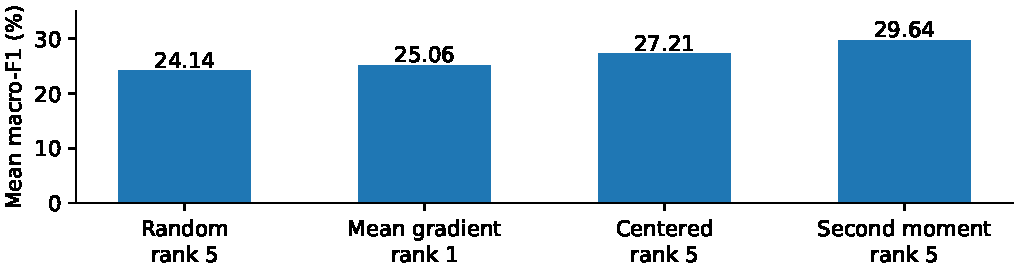
\includegraphics[width=\linewidth]{figures/fig3_basis.pdf}
\caption{\textbf{The choice of visual subspace matters.} Four-event BRIGHT mean macro-F1, compact full lens, $\alpha=3$. Random, centered, and second-moment bases have rank 5; the mean-gradient arm has rank 1. The random result averages three basis seeds; the other constructions use one support configuration. The bars show the recorded means.}
\label{fig:basis}
\end{figure}

The recorded 10,000-resample paired analysis gives a second-moment-minus-centered difference of 0.0243 (95\% interval $[0.0100,0.0388]$) and a second-moment-minus-random difference of 0.0551 ($[0.0058,0.1036]$). The random seed means are 0.2156, 0.2165, and 0.2921, so the benefit is in the observed average, not in excluding every useful random subspace. The separate three-support-seed rank-5 study improves over frozen inference by 0.0457 for the full lens, with reported 95\% interval $[0.0046,0.0847]$. This replication assesses lens-versus-frozen robustness, not a matched three-seed LoRA comparison.

\subsection{Capacity and optimization have non-monotonic effects}
Table~\ref{tab:ablations} changes one factor at a time around the compact rank-5 configuration. Both layers outperform either alone. Increasing rank to 16 helps, whereas rank 32 and doubling support to 48 reduce F1. More capacity or support therefore does not monotonically improve this recipe.

\begin{table}[t]
\caption{\textbf{One-factor BRIGHT sensitivity.} Four-event mean macro-F1, full lens, base rank 5 and $\alpha=3$. Each row is an exploratory sweep; its peak is not substituted into the primary table.}
\label{tab:ablations}
\centering\small
\begin{tabular}{@{}lll@{}}
\toprule
Factor & Values & Corresponding mean macro-F1\\
\midrule
Support & 12 / 24 / 48 & .2538 / .2964 / .2754\\
Layers & 14 / 27 / 14+27 & .1964 / .2213 / .2964\\
Rank & 5 / 8 / 16 / 32 & .2964 / .2972 / .3136 / .2930\\
Updates & 1 / 2 / 4 / 8 & .2486 / .2219 / .2964 / .3048\\
Learning rate & .01 / .05 / .10 / .20 & .2659 / .2964 / .2513 / .2466\\
Bound $\alpha$ & .5 / 1 / 2 / 3 / 5 / 10 & .2384 / .2660 / .2690 / .2964 / .2531 / .2720\\
\bottomrule
\end{tabular}
\end{table}

An all-28-layer rank-16 controller increases the number of coefficients to 14,336 but destabilizes support loss at the sparse controller's learning rate and bound. Reducing both stabilizes Hawaii fitting, yet yields 0.2923 query F1. This is a capacity--optimization interaction, rather than evidence that extra layers are intrinsically harmful. On ManipBench, increasing updates from four to eight improves DROID-pick F1 from 0.2839 to 0.3328 over three seeds. Longer runs continue to alter the result (Appendix~\ref{app:sensitivity}), so the remaining LoRA gap cannot be identified with representational capacity alone.

\section{Why shared directions do not guarantee a useful correction}
\label{sec:mechanism}
We separate coverage of query-loss sensitivity from the utility of a fitted correction. The following probes use query information for mechanism diagnosis, separately from primary adaptation.

\subsection{Energy coverage and signed alignment measure different properties}
Let $G_{Q,j}$ stack the selected query-gradient rows. The coverage statistic is
\begin{equation}
 \rho=\frac{\sum_j\|G_{Q,j}B_{S,j}\|_F^2}{\sum_j\|G_{Q,j}\|_F^2}.
 \label{eq:rho}
\end{equation}
For each module, we also project the token-row mean gradients and compute
\begin{equation}
 \kappa_j=\cos(B_{S,j}^{\top}\bar g_{S,j},B_{S,j}^{\top}\bar g_{Q,j}),\qquad
 \kappa=\frac{\sum_j E_{Q,j}\kappa_j}{\sum_jE_{Q,j}},\quad E_{Q,j}=\|G_{Q,j}\|_F^2.
 \label{eq:kappa}
\end{equation}
We also retain module-level and class-conditional statistics, the latter with class-specific support bases. A direction can carry query energy while its projected mean opposes the support mean.

RoboFail demonstrates the distinction. Its KV energy coverage is 0.7441 on the seed-0 diagnostic, higher than UR5's 0.6862 and RoboVQA's 0.6868, yet its F1 is the lowest of those three runs. Across three seeds, the broader Q/K/V/O aggregate alignment is $0.209\pm0.361$; its sign changes with the support. By contrast, class-conditional success and failure alignments average 0.962 and 0.970. The class-specific sensitivity transfers more consistently than its aggregate mixture.

\begin{figure}[t]
\centering
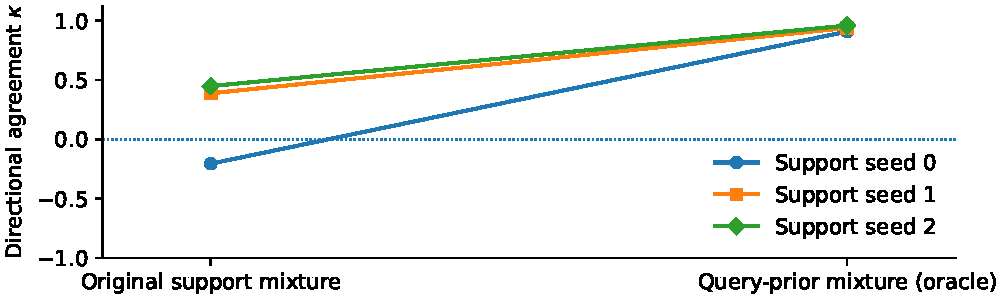
\includegraphics[width=\linewidth]{figures/fig4_mixture.pdf}
\caption{\textbf{Class mixing can reverse an aggregate direction.} RoboFail oracle diagnostic, three support seeds, InternVL3. Reweighting support class means with the query class prior raises the energy-weighted alignment from $0.2092\pm0.3613$ to $0.9340\pm0.0254$, with the same aggregate support basis. Lines connect the same seed. This changes a diagnostic statistic, not the fitted controller or its F1.}
\label{fig:mixture}
\end{figure}

We test the mixing account directly by holding the aggregate support basis fixed and changing only the weights used to combine support class means. For seed 0, balanced support has eight examples per class, whereas query has 116 successes and 21 failures. Reweighting by the query prior changes aggregate alignment from $-0.2065$ to $0.9070$. The change repeats in the other two seeds (Figure~\ref{fig:mixture}). It explains much of the instability in the measured mean direction without requiring each class's geometry to fail. Turning this observation into an adaptation rule would additionally require a usable target-prior estimate and validation against the classification objective.

\subsection{A basis and its intervention are different objects}
Table~\ref{tab:oracles} changes the basis or projection site within each seed-0 task block. Query-derived bases help Camelyon and DROID-pick, but reduce RoboFail F1. Q-only is best on RoboFail and worst among the tested sites on DROID-pick. Thus neither a query-energy basis nor a universal switch to Q explains all outcomes. Broader QKVO interventions change both the location and the coefficient budget, which must be considered when interpreting their gains.

\begin{table}[t]
\caption{\textbf{Basis and site diagnostics.} InternVL3, seed 0, rank 16. Query-basis uses query labels to select $B$, then still fits coefficients on support. Other columns change directly controlled projection outputs. Budgets and inputs are fixed within each task block except for the number of controlled modules.}
\label{tab:oracles}
\centering\small
\begin{tabular}{@{}lrrrrr@{}}
\toprule
Task & KV & Query-basis KV & Q-only & O-only & QKVO\\
\midrule
Camelyon17 & .5994 & .6632 & .5125 & .4172 & \textbf{.6664}\\
RoboFail & .4389 & .4119 & \textbf{.4811} & .4506 & .4538\\
DROID-pick & .2193 & .2482 & .1548 & .1631 & \textbf{.2625}\\
\bottomrule
\end{tabular}
\end{table}

The chain rule clarifies why sensitivity alone is incomplete. At one intervention, let $G_i=\partial\mathcal L_i/\partial\widetilde Z_i$. The gradient of the mixing matrix is
\begin{equation}
 \frac{\partial\mathcal L_i}{\partial A}
 =(Z_iB)^\top(M_i\odot G_i)B.
 \label{eq:controllergrad}
\end{equation}
The actual controller update depends jointly on activations, projected gradients, and optimization. The mean-gradient cosine in Equation~\ref{eq:kappa} omits the activation factor and tokenwise products. It is therefore a diagnostic of agreement, not a descent certificate for the learned matrix. Likewise, a query-gradient eigenspace optimizes energy retention rather than downstream F1. These distinctions explain why high overlap and positive alignment can coexist with a sizeable gap to LoRA under the tested controller.

\section{Related work}
\label{sec:related}
\paragraph{Adaptation at deployment.}
Test-time training constructs a self-supervised objective from unlabeled test inputs \citep{sun2020ttt}. Test-time prompt tuning optimizes prompts using augmented-view consistency and confidence selection \citep{shu2022tpt}. TDA instead maintains an external cache of test features and pseudo-labels \citep{karmanov2024tda}. LoRA-TTT adapts a visual encoder through low-rank updates with reconstruction and entropy objectives \citep{kojima2025lorattt}. Our labeled-support protocol fits one reusable controller before query evaluation. Its LoRA reference is supervised weight adaptation under the same support access, distinct from these unlabeled TTA algorithms.

\paragraph{Weight and representation adaptation.}
LoRA restricts weight updates to low rank while keeping pretrained tensors frozen \citep{hu2022lora}. ReFT demonstrates task-specific low-rank hidden-state interventions \citep{wu2024reft}, and LoFiT selects localized attention representations before learning their adjustments \citep{yin2024lofit}. Our lens restricts the intervention to image-token K/V rows and a support-sensitivity basis. It learns only the mixing matrix within that fixed basis; state selectivity and data-defined directions distinguish the construction.

\paragraph{Correctness-sensitive subspaces and inference control.}
Self-policy distillation identifies capability-relevant KV directions using correctness gradients, applies selective projections during self-generation, and fine-tunes on the generated outputs \citep{hao2026spd}. Our basis construction draws on that sensitivity view, but its purpose is a bounded support-fitted residual reused for an unseen domain's queries. V-Reason optimizes value-cache controllers at inference to guide video reasoning through output-entropy signals \citep{sridhar2026vreason}. Our controller is domain-specific and fixed during each query, with direct supervision supplied by the support labels. These distinctions make the proposed contribution a particular learning formulation for internal visual states, rather than internal intervention in general.


\section{Discussion and limitations}
\label{sec:limitations}
The lens offers a middle ground between fixed inference and broad weight adaptation, with task-dependent benefits.

Three limits bound the present evidence. \emph{First, the primary effect is a fixed-configuration macro-F1 comparison.} BRIGHT uses one support set per event; its balanced accuracy is low, and its three-seed study does not repeat the matched LoRA baseline. Some cross-backbone LoRA references are weak under the short fitting budget. Stronger support-only model selection and independent repeated comparisons remain important for a general accuracy claim. \emph{Second, the intervention has task-dependent utility.} LoRA is substantially stronger on manipulation questions and on the medical F1 comparison. The query-basis and site probes are local diagnostics, not optimization over every possible lens, and do not establish a fundamental capacity barrier. \emph{Third, few-shot estimates remain sensitive to implementation and sampling.} Loss scaling and answer-span conventions differ across task and BRIGHT paths; spatially concentrated support and one nominally identical Hawaii repeat differing by 0.0338 F1 motivate stricter replication. The reported timings cover the compact rank-5 lens, not the rank-16 primary controller.

A visual lens transforms internal evidence; it neither increases image resolution nor establishes that the base model already has the complete task capability. Controlled image interventions can next separate visual-evidence gains from changes in class priors or answer scoring, addressing the difference between macro-F1 and BA.

\section{Conclusion}
\label{sec:conclusion}
We introduced a learned visual lens: a support-conditioned, low-rank residual on visual K/V states inside a frozen VLM. Correct-answer gradients select the linear subspace, and a bounded controller learns the domain-specific transformation. The primary disaster comparison achieves 32.08\% mean macro-F1 with 1,024 learned coefficients, versus 29.86\% for the fixed-duration 10.1M-parameter LoRA reference. Cross-task controls distinguish energy coverage, directional agreement, and the realized effect of an intervention. The central result is a concrete alternative for few-shot adaptation: useful change can be localized in internal visual states, with its benefits determined by the task, representation, and fitted correction rather than parameter count alone.
\label{maintextend}

\clearpage
\section*{AI use statement}
Generative AI tools assisted the research discussions, experiment-code development, source retrieval, manuscript drafting, and figure-production scripts. Numerical results in this draft are taken from executed experiment reports; the writing and plotting process did not generate new experimental measurements. The conceptual method diagram is a schematic, while numerical plots reproduce recorded values. Final validation of the research artifacts and approval of the submission are the authors' responsibility.

\section*{Ethics statement}
The experiments use existing research datasets and evaluate offline predictions. The learned controllers are not validated for medical diagnosis, autonomous disaster-response allocation, or safety-critical robot control. Deployment in those settings requires task-specific evaluation, human oversight, and compliance with the datasets' access and use conditions. No new human-subject data were collected for the reported comparisons.

\section*{Reproducibility statement}
Appendix~\ref{app:protocol} specifies preprocessing, supervision, optimization budgets, and the separation of deployment estimates from query-information diagnostics. All tables retain their reported seed and configuration scopes. The accompanying plotting assets regenerate the numerical figures from the attributed data values. Prediction-level manifests, model checkpoints, and full experiment artifacts are needed for independent model-run replication and paired statistical reanalysis.

\bibliographystyle{iclr2027_conference}
\bibliography{references}

\clearpage
\appendix
\section{Properties of the residual operator}
\label{app:proof}
\paragraph{Energy-retention proof.}
Write $C=U\Lambda U^\top$, with eigenvalues sorted in descending order, and let $H=U^\top B$. Since $H^\top H=I_r$,
\begin{equation}
 \tr(B^\top CB)=\sum_{k=1}^{d}\lambda_k\|H_{k,:}\|_2^2.
\end{equation}
The row weights lie in $[0,1]$ and sum to $r$. The weighted sum is maximized by assigning weight one to the largest $r$ eigenvalues and zero to the rest, which is attained by the corresponding eigenvectors. The equality to $N^{-1}\sum_i\|G_iB\|_F^2$ follows by cycling the trace. Multiplying $C$ by a positive scalar changes eigenvalues but not the selected eigenspace.

\paragraph{Identity and residual bound.}
For $R=0$, $A=0$ and $\widetilde Z=Z$. For finite $R$, $\|A\|_2\leq\|A\|_F=\alpha\|R\|_F/(1+\|R\|_F)<\alpha$. Since $B^\top B=I$, multiplying by $B^\top$ preserves the Frobenius norm of the low-dimensional residual, giving Equation~\ref{eq:bound}. The residual is entirely in $\operatorname{span}(B)$; the part orthogonal to that span is unchanged at the edited site. Later layers can amplify, suppress, or redirect its effect.

\paragraph{Controller gradient.}
Set $U=ZB$ and $\widetilde Z=Z+M\odot UAB^\top$. For the upstream gradient $G$,
\begin{equation}
 d\mathcal L=\tr\left(G^\top[M\odot U(dA)B^\top]\right)
 =\tr\left([U^\top(M\odot G)B]^\top dA\right).
\end{equation}
This yields Equation~\ref{eq:controllergrad}. Across support examples, the terms add with the weights of Equation~\ref{eq:fit}. The derivative through the norm-bounded parameterization and the optimizer further determine the realized update in $R$. At zero initialization, the first-order derivative of $A$ with respect to $R$ is multiplication by $\alpha$.

\paragraph{Relation to weight updates.}
For an unmasked linear projection $Z=HW$, the residual can be written as $H(W+WBAB^\top)$, with $\operatorname{rank}(WBAB^\top)\leq r$. Thus the distinction is not a claim that all state transformations lie outside weight-space representations. The present lens constrains the update through a fixed, support-derived basis and applies it only to selected token rows. A shared projection-weight update would act on all rows; the token mask makes the lens conditional on their visual role.

\section{Detailed protocol and accounting}
\label{app:protocol}
\begin{table}[!ht]
\caption{\textbf{The complete adaptation procedure.} The query set is absent from both learning stages.}
\label{tab:algorithm}
\centering
\begin{tabularx}{\linewidth}{@{}r X@{}}
\toprule
1 & Freeze the pretrained VLM and select decoder K/V projections and visual mask.\\
2 & For each labeled support example, backpropagate its answer-span loss and accumulate $G_{i,j}^{\top}G_{i,j}$.\\
3 & Extract $B_j$ using Equation~\ref{eq:basis}; initialize every $R_{e,j}=0$.\\
4 & Repeat the specified number of full-support Adam updates on Equation~\ref{eq:fit}, with fixed bases and backbone.\\
5 & Save bases and coefficients. Score each query with the same fixed lens.\\
\bottomrule
\end{tabularx}
\end{table}
\begin{table}[!ht]
\caption{Implementation settings for the reported experiment blocks. ``Full-support update'' accumulates all support losses before an optimizer step.}
\centering\small
\begin{tabularx}{\linewidth}{@{}l X X@{}}
\toprule
Block & Visual lens & LoRA\\
\midrule
Primary BRIGHT & Full $r16$, layers14/27, $\alpha3$, Adam, 4 full-support updates, lr .05, mean loss + .001 penalty & $r16$, scaling32, dropout.05, QKVO, lr $10^{-4}$, batch1/accum3, 8 updates\\
Extra BRIGHT & Same lens; backbone-specific processor & Same adapter settings, lr $2\cdot10^{-4}$, one support24 pass/accum3\\
Camelyon / ManipBench & Full $r16$, $\alpha3$, 4 updates, lr .05, summed loss + .001 penalty & Four passes, batch1, lr $2\cdot10^{-4}$, 64/128 updates for support16/32\\
Guardian baseline & Full $r16$, $\alpha3$, 4 updates, lr .05 & Four passes on support16; 64 updates\\
Guardian follow-up & Full $r16$, $\alpha3$, 8 updates, lr .01 & Same baseline as preceding row\\
\bottomrule
\end{tabularx}
\end{table}

\paragraph{Input construction.}
BRIGHT retains the original pre/post-image order and dataset metadata, with crops taken around each building. Camelyon is a hospital-2 few-shot derivative of WILDS. Its three support manifests share the locked query subset. ManipBench preserves the question and candidate order within each example. Guardian composites before/after observations into one vertical image and holds out the selected support from its query complement separately for each seed. The lens covers all visual rows of that composite, rather than an unimplemented after-only mask.

\paragraph{Answer likelihood.}
For candidate $c$, $s_c=\sum_{u\in\mathcal T_c}\log p(c_u\mid x,c_{<u})$ and $p_c=\sm(s)_c$. Scores are not normalized by candidate length. Support training uses the model's mean token loss on the designated answer span. The corrected InternVL single-image path includes the common \texttt{Answer:} prefix in that span. This prefix is shared across candidate completions and leaves exact-arithmetic within-example ranking unchanged, but contributes to support gradients as well as their scale. Input resizing, tokenizer behavior, and mask groups must be identical across methods in a block.

\paragraph{Replication and inference.}
A support seed describes sampling of the adaptation set, not a new pretrained model. The recorded BRIGHT bootstrap/permutation analyses use 10,000 resamples under their paired event/query procedure. They are separate from a fresh group-aware confidence analysis. Repeated query examples across support seeds must not be counted as independent test instances. Primary rank16, compact rank5, and oracle rows have distinct statistical units and are kept separate.

\begin{table}[!ht]
\caption{\textbf{Measured compact-controller efficiency.} One RTX 3090, Hawaii query300. Adaptation time is excluded from the query timing.}
\label{tab:efficiency}
\centering\small
\begin{tabular}{@{}lrrrr@{}}
\toprule
Method & Seconds/query & Peak MiB & Learned scalars & Stored adapter\\
\midrule
Frozen & 1.3405 & 17,470 & 0 & --\\
LoRA & 1.3725 & 17,508 & 10,092,544 & $\sim39.5$ MiB\\
Full lens, rank5 & 1.3382 & 17,470 & 100 & $\sim44$ KiB\\
Diagonal lens, rank5 & 1.3384 & 17,470 & 20 & $\sim44$ KiB\\
\bottomrule
\end{tabular}
\end{table}

\section{Additional task metrics}
\label{app:tasks}
\begin{table}[!ht]
\caption{\textbf{Qwen3-VL task comparison.} Three-support-seed macro-F1 mean $\pm$ sample SD. Lens uses the four-update task setting.}
\centering\small
\begin{tabular}{@{}lrrrr@{}}
\toprule
Task & Frozen & LoRA & Random-KV & Full lens\\
\midrule
Camelyon17 & $.3407\pm.0000$ & $\mathbf{.6857\pm.2026}$ & $.3922\pm.0039$ & $.5857\pm.0902$\\
Bridge pick & $.7006\pm.0000$ & $\mathbf{.8567\pm.0304}$ & $.7004\pm.0012$ & $.7388\pm.0146$\\
DROID arti. & $.5072\pm.0000$ & $\mathbf{.7860\pm.0409}$ & $.5187\pm.0024$ & $.5959\pm.0139$\\
DROID pick & $.5202\pm.0000$ & $\mathbf{.7624\pm.0145}$ & $.5279\pm.0017$ & $.5760\pm.0045$\\
\bottomrule
\end{tabular}
\end{table}

\begin{table}[!ht]
\caption{\textbf{Corrected InternVL task metrics.} Frozen / LoRA / full lens / random basis, in that order. All are three-seed means under the four-update lens setting.}
\centering\small
\begin{tabular}{@{}lll@{}}
\toprule
Task & Balanced accuracy & NLL\\
\midrule
Camelyon17 & .5000 / .6956 / .5689 / .5578 & .9693 / 1.9900 / .7841 / .7276\\
Bridge pick & .2500 / .5575 / .3142 / .2483 & 1.6049 / 3.4351 / 1.4500 / 1.5296\\
DROID arti. & .1675 / .6775 / .3367 / .1775 & 1.7993 / 2.2237 / 1.4513 / 1.7158\\
DROID pick & .1650 / .4625 / .2958 / .1958 & 1.8426 / 2.6912 / 1.4663 / 1.6881\\
\bottomrule
\end{tabular}
\end{table}

\paragraph{Guardian likelihood and class-conditional control.}
The four-update lens has NLL 0.7734, 0.8340, and 0.8158 on UR5, RoboFail, and RoboVQA, compared with 3.0313, 7.5011, and 4.3961 for LoRA. These values belong to the four-update baseline, not the eight-update follow-up. A RoboFail seed-0 probe using a separate support-class lens to score each candidate obtains F1 0.1625 and BA 0.4306, with success recall 0.0517 and failure recall 0.8095. Independently adapted candidate scores require a common comparison rule; this probe supplies no evidence for a useful class-conditional extension.

\section{Sensitivity and diagnostic scope}
\label{app:sensitivity}
\begin{table}[!ht]
\caption{\textbf{Full rank-16 residual-bound sweep.} BRIGHT macro-F1. The per-event maxima use query outcomes and remain exploratory.}
\centering\small
\begin{tabular}{@{}lrrrrrr@{}}
\toprule
Event & $\alpha=.5$ & 1 & 2 & 3 & 5 & 10\\
\midrule
Hawaii & .2622 & .3338 & .3869 & .2957 & .3239 & .3476\\
Libya & .3249 & .2760 & .3852 & .3739 & .3394 & .2943\\
Noto & .2354 & .3270 & .3095 & .3112 & .3021 & .2770\\
Turkey & .2627 & .1876 & .2527 & .3025 & .2472 & .2578\\
\bottomrule
\end{tabular}
\end{table}

\begin{table}[!ht]
\caption{\textbf{Optimization follow-up on InternVL DROID-pick.} Multi-seed means are distinguished from seed-0 screens. These are not a controlled steps-only sweep when learning rate changes.}
\centering\small
\begin{tabular}{@{}rrlr@{}}
\toprule
Updates & Learning rate & Replication & Macro-F1\\
\midrule
4 & .05 & Three seeds & $.2839\pm.0729$\\
8 & .05 & Three seeds & $.3328\pm.0948$\\
16 & .01 & Three seeds & $.3347\pm.1153$\\
32 & .01 & Seed 0 & .3438\\
64 & .01 & Seed 0 & .3984\\
64 & .02 & Seed 0 & .4147\\
\bottomrule
\end{tabular}
\end{table}

\begin{figure}[!ht]
\centering
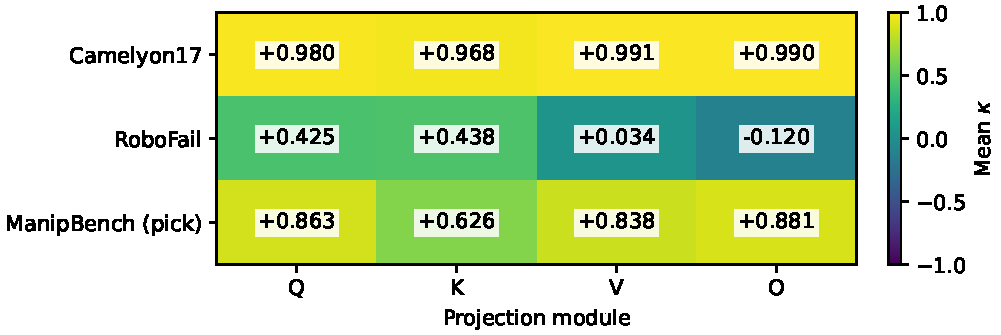
\includegraphics[width=\linewidth]{figures/figA_module_alignment.pdf}
\caption{\textbf{Directional agreement depends on the projection.} Three-support-seed means of the query-label diagnostic. Q/K/V/O are analyzed separately; the plotted entries are not the aggregate cosine. Negative and positive values are annotated explicitly.}
\label{fig:module}
\end{figure}

\paragraph{Energy and direction use different aggregation.}
The selected token gradients are concatenated before the per-module mean is computed. Class-conditional rows refit the basis using the support examples of that class; their alignment is therefore not measured in the same basis as every aggregate row. The query-prior probe instead fixes the aggregate basis and changes only the mixture of support class means. These choices isolate different questions and must not be interchanged when interpreting a sign reversal.

\paragraph{BRIGHT geometry.}
The archived paired-image geometry probe uses support12 and a balanced query300 derivative. Its Q/K/V/O aggregate $(\rho,\kappa)$ is $(.4328,.9754)$ on Hawaii and $(.3689,.6769)$ on Libya. These are qualitative checks on separate folds, not points paired to the support24 primary performance for a predictive correlation.

\end{document}
